\section{Curves and parametric descriptions}

A curve can be described in different ways. One way is to give an equation such as
\[
y=f(x).
\]
For example, \(y=x^2\) describes a parabola in the plane.

Another way is to use a parameter. A parameter is an additional variable that describes how the coordinates are generated.

\begin{definitionbox}
A parametric curve in the plane can be written as
\[
\mathbf{r}(t)=(x(t),y(t)).
\]
As \(t\) changes, the point \((x(t),y(t))\) moves along the curve.
\end{definitionbox}

For example, the equations
\[
x=t, \qquad y=t^2
\]
give the same parabola as \(y=x^2\), because the moving point is
\[
(x,y)=(t,t^2).
\]

Another important example is
\[
\mathbf{r}(t)=(\cos t,\sin t).
\]
This describes the unit circle, because
\[
\cos^2 t+\sin^2 t=1.
\]

\begin{center}
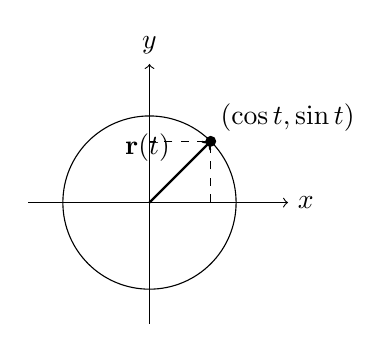
\begin{tikzpicture}[scale=1.1]
    \draw[->] (-1.4,0) -- (1.6,0) node[right] {$x$};
    \draw[->] (0,-1.4) -- (0,1.6) node[above] {$y$};
    \draw (0,0) circle (1);
    \draw[->, thick] (0,0) -- ({cos(45)},{sin(45)}) node[midway, above left] {$\mathbf{r}(t)$};
    \fill ({cos(45)},{sin(45)}) circle (1.8pt);
    \draw[dashed] ({cos(45)},0) -- ({cos(45)},{sin(45)}) -- (0,{sin(45)});
    \node[above right] at ({cos(45)},{sin(45)}) {$(\cos t,\sin t)$};
\end{tikzpicture}
\end{center}

\begin{remarkbox}
At this stage, \(t\) is only a mathematical parameter. The important idea is that a curve can be described by giving its coordinates as functions of one parameter.
\end{remarkbox}
